\documentclass[12pt]{article}
\setcounter{secnumdepth}{0}
\usepackage[margin=1in]{geometry} 
\usepackage{amsmath,amsthm,amssymb}
\usepackage{hyperref}
\usepackage{listings}
\usepackage{color}
\usepackage{advdate}
\definecolor{dkgreen}{rgb}{0,0.6,0}
\definecolor{gray}{rgb}{0.5,0.5,0.5}
\definecolor{mauve}{rgb}{0.58,0,0.82}
\usepackage{graphicx}
\hypersetup{
    colorlinks,
    citecolor=black,
    filecolor=black,
    linkcolor=black,
    urlcolor=blue
}

\lstset{frame=tb,
  aboveskip=3mm,
  belowskip=3mm,
  showstringspaces=false,
  columns=flexible,
  basicstyle={\small\ttfamily},
  numbers=none,
  numberstyle=\tiny\color{gray},
  keywordstyle=\color{blue},
  commentstyle=\color{dkgreen},
  stringstyle=\color{mauve},
  breaklines=true,
  breakatwhitespace=true,
  tabsize=3,
  emph={  
    enterCS,
    releaseCS,
    haveResource
    },
  emphstyle={\color{dkgreen}\bfseries}
}
\begin{document}
\title{CS3563: DBMS II\\Assignment 3}
\author{Sagar Jain\\CS17BTECH11034}
\date{\AdvanceDate[-1]\today}
\maketitle
\section{Solutions}
\begin{enumerate}
\item
\begin{enumerate}
\item  
\begin{align*}
	size &= (\# recording\;surfaces) * (\#tracks/surface) * (\#sectors/track)*(size\;of\;sector)\\
	&= 8 * 8192 * 512 * 512\;B\\
	&= 17179869184\;B \\
	&= 16 \;GB
\end{align*}
\item The last given address is \textbf{$<$3, 4095, 127$>$}. With this information it can be assumed that all there might be some data on the addresses before and including the one given which we would not want to overwrite.\\
Each surface has 8192 tracks. Ideally, we would want to start storing a new file in a new track, unless the file is smaller than the size remaining in the track in which the read-write head is currently, this is so that we can decrease the totoal number of tracks over which the file is spread, this will reduce the total time needed to access the file as we reduce the total movement of the disk arm, therefore reducing the seek time. Another consideration is that for the fastest read-write time we could store it in the same cylinder over different platters. So we start storing on cylinder 4096 on surface 3, then move onto surfaces 4,5,6,7 and then begin on the cylinder 4097 and so on.
Assuming that an 1 MB = 1024 KB and 1KB = 1024 B, the number of sectors needed would be,\\\\
$ fileSize\;/\;trackSize = (1000*1024*1024)/(512*512)= 4000\; tracks$\\\\
We have 5 recording surfaces available, that would mean 4000/5=800 cylinders.\\
\\So, if we begin at the address \textbf{$<$3, 4096, 0$>$}, the last sector of the file would be stored at \textbf{$<$7, 4895, 511$>$}.
\item There are 4000 tracks which need to be read completely. So that is 4000 rotations, also the read-write would have to move 800 times when it is moving to the next track. An assumption I am making here is that the file can be read backwards and assembled by the disk controller or other operating system utility. So the total time required would be:\\
\begin{align*}
RPS &= RPM/60\\
&=7200/60\\
&=120\\
Time\;to\;read\;one\;track &= 1/RPS\\
&=1/120\\
seekTime &= 5ms\\
Total\;time &= 3999*5/1000 + 4000/120\\
&=53.328
\end{align*}
If the file can only be read from the beginning to the end we would have to seek to the beginning initially that would increase the total time by 5ms + 1/120s = 8.3ms (moving disk arm \& rotating to the beginning of the track), in that case the total time would be \textbf{53.342s}.\\
\item Assuming the file was read from beginning to end, the head would be on track 8095 after reading the file.\\\\
For FCFS, the order of the tracks visited and total distance would be as follows:\\\\
\begin{tabular}{ | l | l | }
\hline
	Track Number & Distance \\ \hline
	8095 &  \\ \hline
	200 & 7895 \\ \hline
	5000 & 4800 \\ \hline
	4200 & 800 \\ \hline
	5 & 4195 \\ \hline
	7200 & 7195 \\ \hline
	4000 & 3200 \\ \hline
	2200 & 1800 \\ \hline
	800 & 1400 \\ \hline
	6500 & 5700 \\ \hline
	Total Distance & 36985 \\ \hline
\end{tabular}\\\\\\
The total distance travelled by the disk arm would be 36985, in terms of number of cylinders when using the FCFS algorithm.\\\\\\\\\\\\
Using the elevator algorithm the following would be the order and the distance travelled.\\\\
\begin{tabular}{ | l | l | }
\hline
	Track Number & Distance \\ \hline
	8095 &  \\ \hline
	7200 & 895 \\ \hline
	6500 & 700 \\ \hline
	5000 & 1500 \\ \hline
	4200 & 800 \\ \hline
	4000 & 200 \\ \hline
	2200 & 1800 \\ \hline
	800 & 1400 \\ \hline
	200 & 600 \\ \hline
	5 & 195 \\ \hline
	Total Distance & 8090 \\ \hline
\end{tabular}\\\\\\
The total distance travelled by the disk arm would be 8090, in terms of number of cylinders when using the elevator algorithm.
\end{enumerate}
\item \begin{enumerate}
\item
\textbf{Insert A}\\\\
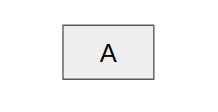
\includegraphics[scale=0.6]{q31.png}\\
\textbf{Insert C}\\\\
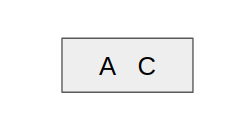
\includegraphics[scale=0.6]{q32.png}\\
\textbf{Insert E}\\\\
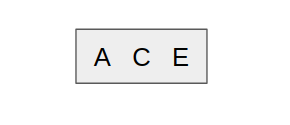
\includegraphics[scale=0.6]{q33.png}\\\\\\\
\textbf{Insert G}\\
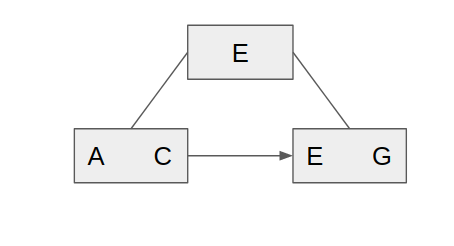
\includegraphics[scale=0.5]{q34.png}\\
\textbf{Insert I}\\
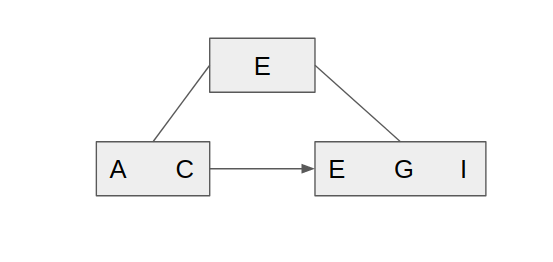
\includegraphics[scale=0.5]{q35.png}\\
\textbf{Insert B}\\
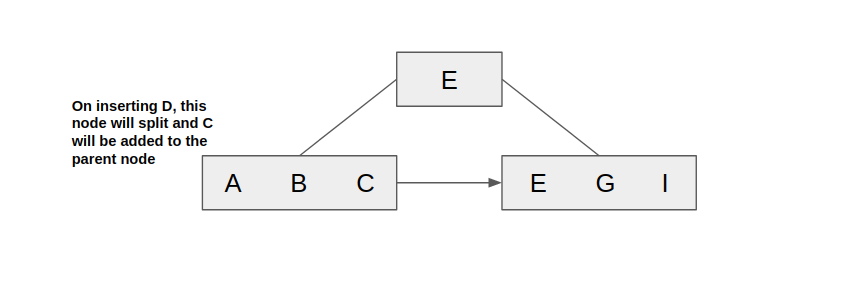
\includegraphics[scale=0.5]{q36.png}\\
\textbf{Insert D}\\
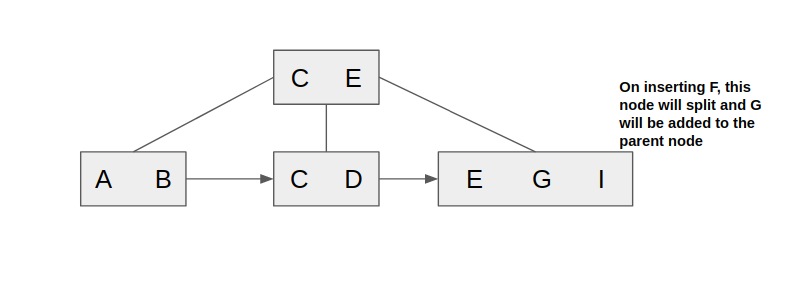
\includegraphics[scale=0.5]{q37.png}\\\\\\\\
\textbf{Insert F}\\
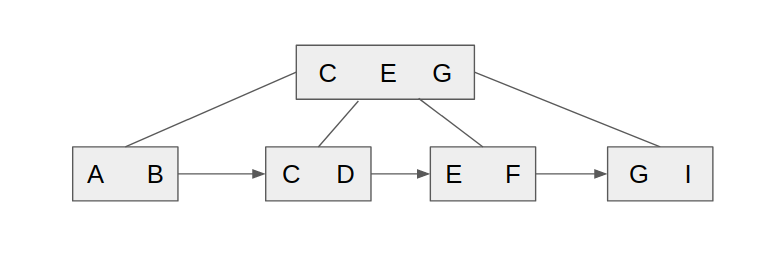
\includegraphics[scale=0.55]{q38.png}\\
\textbf{Insert H}\\
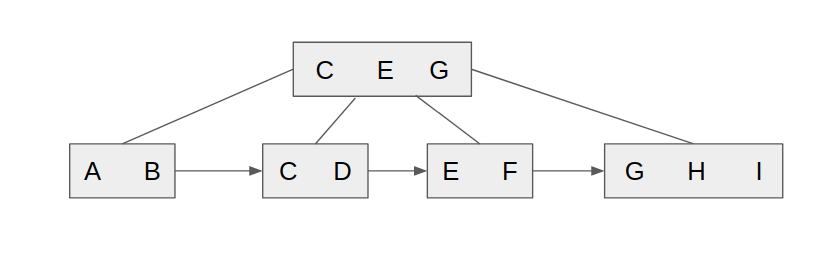
\includegraphics[scale=0.55]{q39.png}\\
\textbf{Insert J}\\
On inserting \textbf{J}, the node with \textbf{$<$G, H, I$>$} will split and \textbf{I} will be pushed to the parent node, but then the parent node will have four keys, so it will split too, this will push \textbf{G} again upwards to create a new parent node. \\
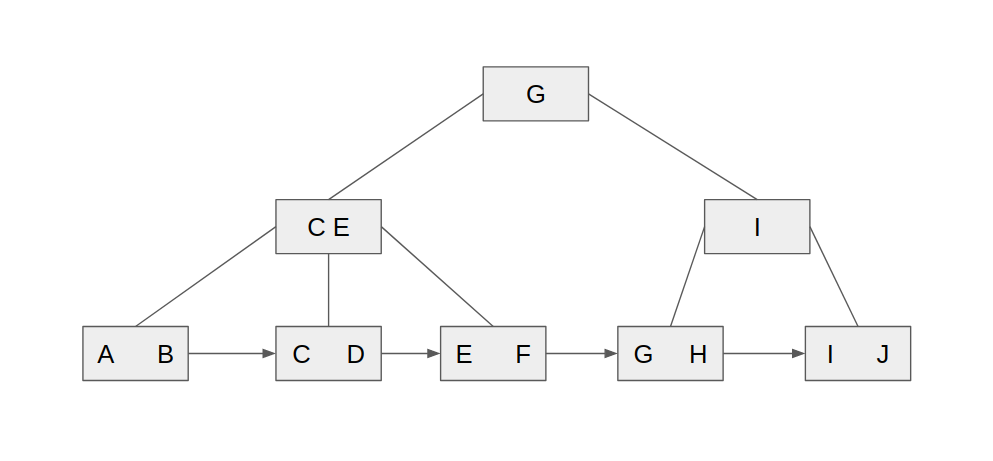
\includegraphics[scale=0.49]{q310.png}\\\\
\item 
\textbf{delete I}\\
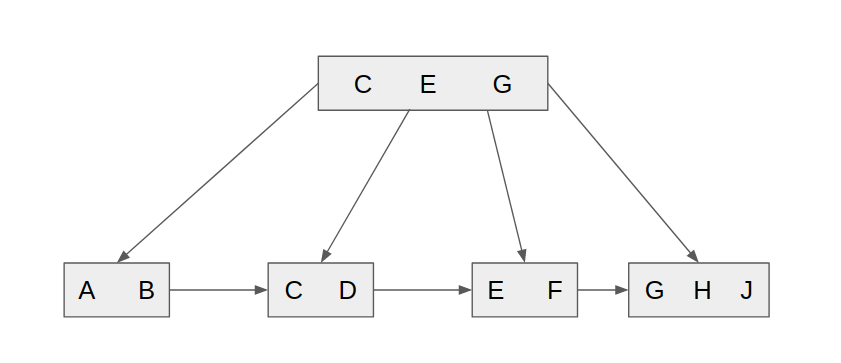
\includegraphics[scale=0.5]{2b1.png}\\
\textbf{delete G}\\\\
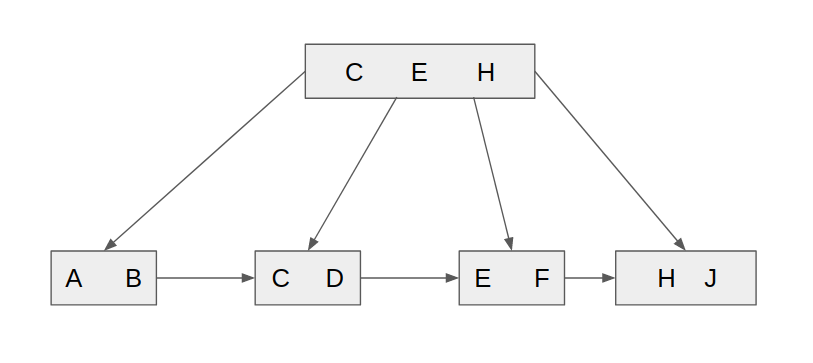
\includegraphics[scale=0.5]{2b2.png}\\
\textbf{delete H}\\\\
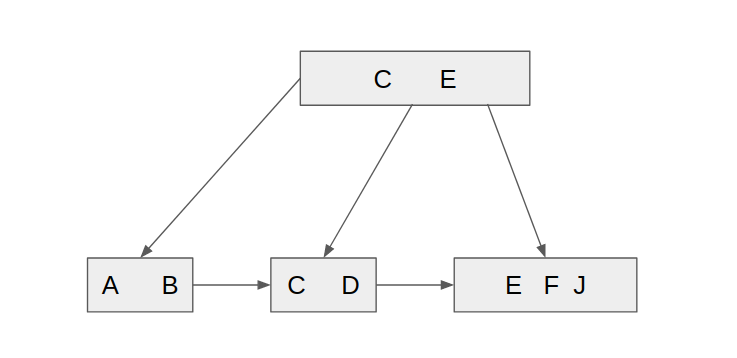
\includegraphics[scale=0.5]{2b3.png}\\
\end{enumerate}
\item ~\\ 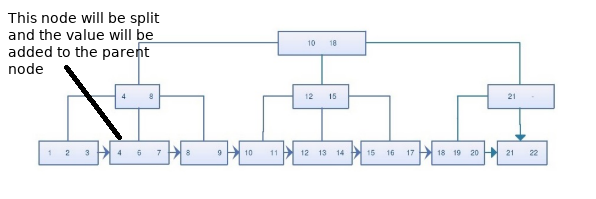
\includegraphics[scale=0.8]{i1e.png}\\\\
After inserting data entry with key 5 into the tree it would like the following:\\
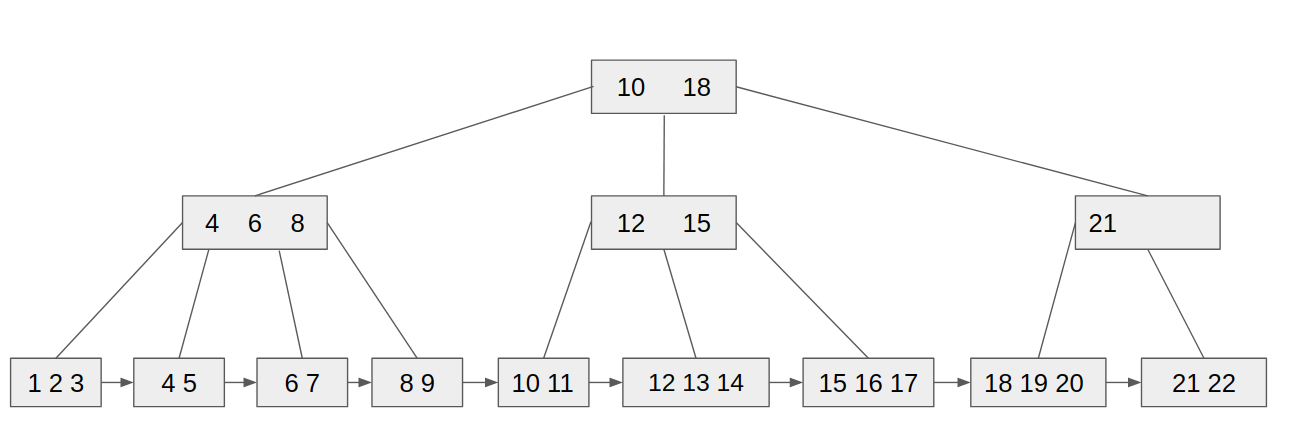
\includegraphics[scale=0.35]{q3.png}
\item \begin{enumerate}
\item Index records have the search key value and the assciated pointer, so the size of an index records would the sum of the sizes of the two, i.e. $45 + 15 = 60\;bytes$. The number of pointers in a single node would be the same as the number of index records that can be stored in a single disk page. We have 30,000 records and the size of a disk page is 1500 bytes. So, the number of index records in a single node is 1500/60=25, but leaf nodes need extra space for next node pointer so we can have 24 records per node. Since the nodes at each level are filled as much as possible, the number of levels in the B+ tree is $ceil(log(30000/24)) = 4$
\item Level 1: 1 node (root)\\
Level 2: 3 nodes\\
Level 3: 53 nodes\\
Level 4: 1250 nodes
\item If the size of key is reduced to 10 bytes then we could have 59 index records in each node. So the number of levels in the B+ tree would be $ceil(log(30000/59)) = 3$.
\item If each page in only 70\% full then the number of index records in each node would be 17 since $17*60 + 10 < 70*1500/100 < 18*60 + 10$ . So the number of levels in the B+ tree would be $log(30000/17) = 4$
\end{enumerate}
\item The algorithm used for extendible hashing is the one found \href{https://www.geeksforgeeks.org/extendible-hashing-dynamic-approach-to-dbms/}{here}.\\ 
We start of with the global depth equal to 1. We have two buckets initially and both have local depth equal to 1. \\
We use the LSBs of the hashed value to compute the bucket into which the value has to be stored.\\
The following images show in a step wise manner the insertion of elements into the hashtable.\\\\
\textbf{Insert 7}\\\\
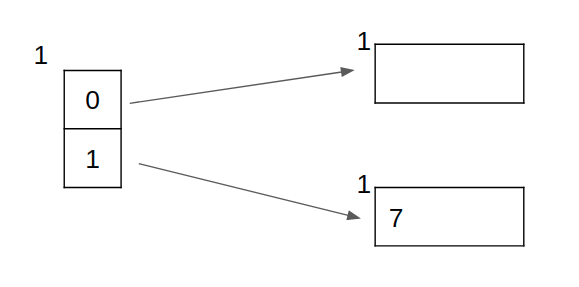
\includegraphics[scale=0.53]{51a.png}\\
\textbf{Insert 8}\\\\
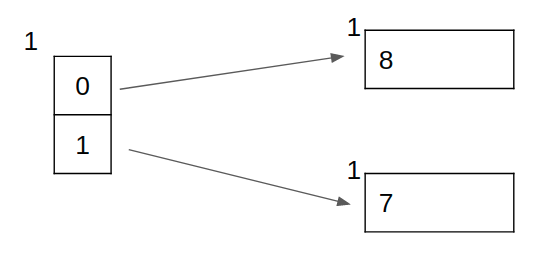
\includegraphics[scale=0.53]{51b.png}\\
\textbf{Insert 10}\\\\
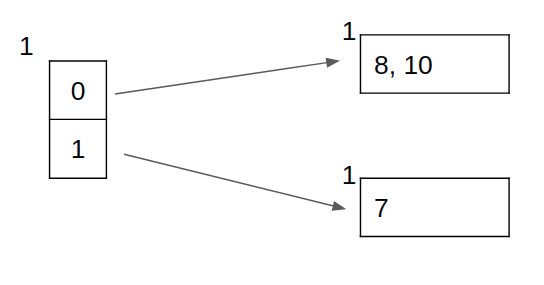
\includegraphics[scale=0.53]{52a.png}\\
\textbf{Insert 11}\\
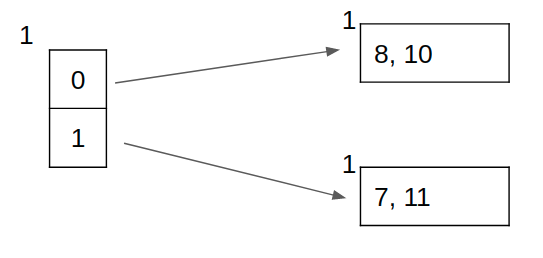
\includegraphics[scale=0.5]{52b.png}\\
\textbf{Insert 15, 16}\\
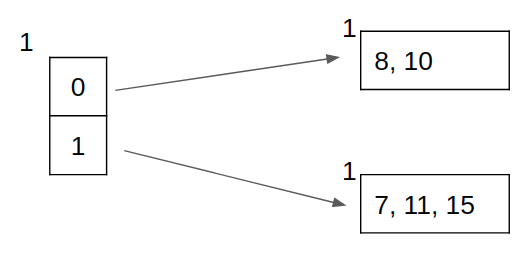
\includegraphics[scale=0.5]{53a.png}\\
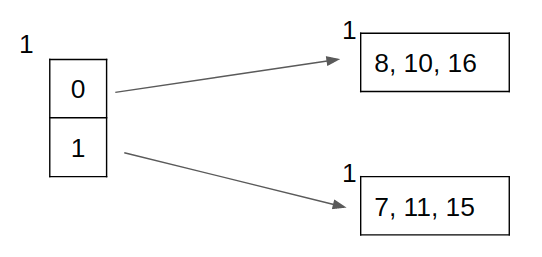
\includegraphics[scale=0.5]{53b.png}\\
On \textbf{inserting 17}, there will be a bucket split in the second bucket. Global depth will become four. Now we will have, two with depth two and one with depth one.\\
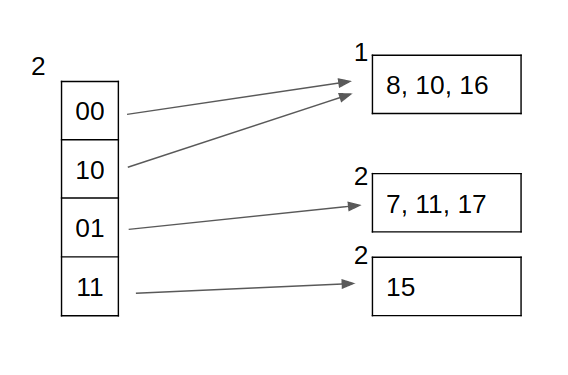
\includegraphics[scale=0.5]{54.png}\\
On \textbf{inserting 19} once again there will be a bucket split in the second bucket.\\
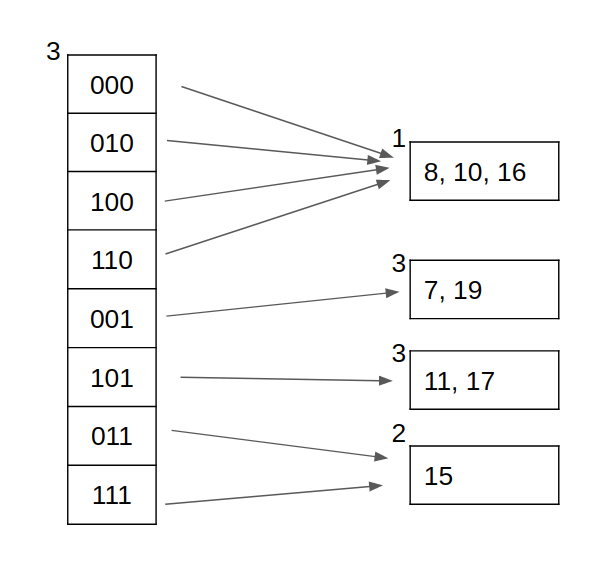
\includegraphics[scale=0.48]{55.png}\\
On \textbf{inserting 33, 53} there will be no split, but on \textbf{inserting 58}, we will have to split the first bucket. Then all the values will have to be rehashed and we would consider the last two bits of the values to decide which bucket to put them in.\\
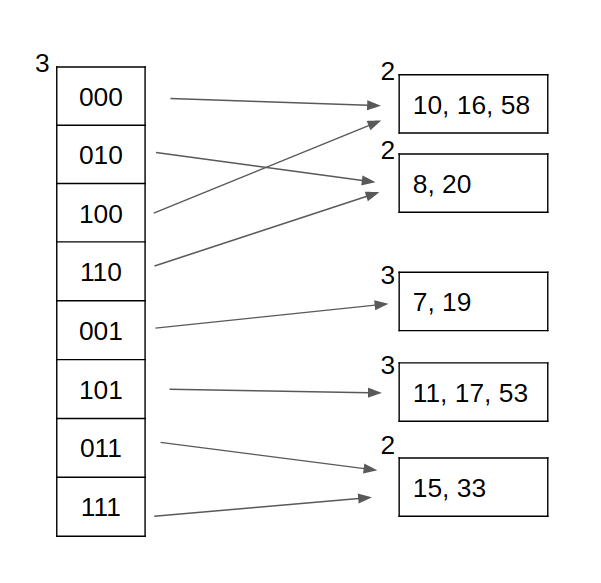
\includegraphics[scale=0.5]{56.png}
\end{enumerate}
\end{document}